%!TEX root = mainfile.tex

\section{The Gunn-Peterson Effect} % (fold)
\label{sec:the_gunn_peterson_effect}
	The current theoretical description of cosmic evolution at the end of the dark ages of the universe has gained widespread acceptance; as have the qualitative stages and processes of the epoch of reionisation. However, real empirical evidence from these eras remains sparse and clouded by large uncertainties. To accept the popular descriptions as fact without recourse to solid and quantitative evidence would be premature and in order to effectively investigate these high-redshifts, it is necessary to understand the spectral features of the objects we see in them.

	Along with measurements of the Hydrogen \SI{21}{\centi\metre} line, the Gunn-Peterson effect and its impact on the spectra of distant galaxies are the two primary methods of observation currently being used to throw light on the epoch of reionisation and the early universe as a whole.

	\subsection{The Lyman Break} % (fold)
	\label{sub:the_lyman_break}
		The Lyman-$\alpha$ line is the spectral line corresponding to the $n=1$ to $n=2$ electron level transition in neutral Hydrogen; it is the first transition in the Lyman series and the lowest energy level transition a Hydrogen atom is capable of undergoing from its ground state. This transition is of particular relevance to cosmology and cosmic reionization, firstly, because during primordial nucleosynthesis, Hydrogen atoms were created in the greatest abunance, with over 90\% of the produced atoms being Hydrogen, approximately 8\% being Helium with smaller abundancies of other light elements. Furthermore, during the epoch of reionization the average time between atomic excitations was large compared to the decay times of the excited states, meaning that the vast majority of HI atoms were in the ground state. This meant that the neutral IGM was highly resonant with photons of Lyman-$\alpha$ frequency, and was largely incapable of absorbtion of lower freqencies (ignoring the effects of fine and hyperfine line splitting).

		The proportion of radiation of some frequency which penetrates a medium is characterised by the medium's optical depth, $\tau$, for that wavelength, such that:
		\begin{align}
			I = I_0 e^{-\tau}.
		\end{align}
		The optical depth of neutral Hydrogen to Lyman-$\alpha$ photons can be approximated by
		\begin{align}
			\tau_{GP} = 3.6 \times 10^5	\left ( 	\frac{\Omega_m h^2}{0.13}	\right ) ^{-1/2}
										\left ( 	\frac{\Omega_b h^2}{0.02}	\right )
										\left ( 	\frac{1+z}{7}			\right )^{3/2}
										\left ( 	\frac{n_{HI}}{n_H}			\right ) .
		\end{align}
		The full derivation of this formula is given in Appendix~\ref{app:derivation_of_the_gunn_peterson_optical_depth}.

		Using conventional values for $\Omega_b$ and $\Omega_m$ it can be shown that, for redshifts $>6$, the fraction of neutral Hydrogen required to reduce the transmitted intensity to less than 1\% of the incident value is of the order of $10^{-5}$. Therefore, only a small amount of neutral Hydrogen must occupy the intervening space between the distant galaxy and the observer to effectively eliminate the Lyman-$\alpha$ frequency from the object's spectrum.

		However, the frequency  of the absorbed radiation is not the Lyman-$\alpha$ line in the rest frame of the emitter, but in the rest frame of the absorber, such that as the light travels along its path to the observer successively shorter and shorter wavelengths are redshifted into resonance with the local neutral IGM and each wavelength is, in turn, scattered into extinction. This process continues untill the radiation reaches a region of spacetime where the Hydrogen neutral fraction is significantly below the previously calculated value of $10^{-5}$.

		This effect, discovered by Gunn and Peterson in 1965, results in the extinction of a large portion of the flux from distant galaxies in the region blueward of the object's rest frame  Lyman-$\alpha$ line, known as the Lyman-$\alpha$ break, or the Gunn-Peterson trough.
		\begin{figure}[htbp]
			\centering
			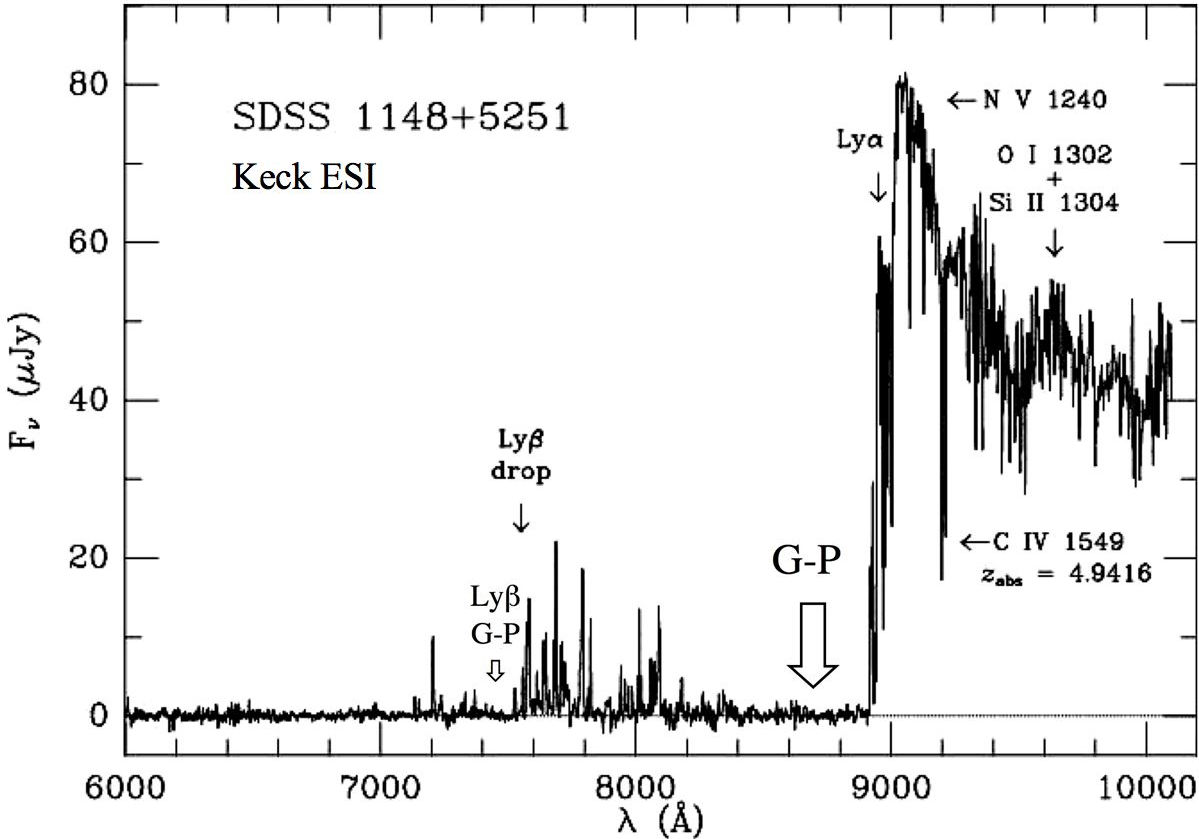
\includegraphics[width=0.6\textwidth]{../Images/dropout.jpg}
			\caption{Gunn-Peterson dropout in the spectrum of a galaxy at $z=6.4$.}\label{fig:dropout}
		\end{figure}

		The spectral flux from distant galaxies redward of the Lyman break is unaffected by Gunn Peterson scattering and remains representative of the true brightness of the luminous object, while the region of the spectrum blueward of the break is highly obscured by the scattering effect of neutral hydrogen. While the portion of the true emitted spectrum in this region is lost, the extent of the loss contains infomation regarding the optical depth of the intervening space and, thereby, the density of neutral hydrogen at the redshift at which the Lyman break falls on that wavelength. Moreover, because the Lyman alpha line invariably falls at a specific point in the emitted spectrum, the redshift of any observed spectrum with an identifiable Lyman break can be measured easily. The break is such a strong spectral feature that it can be located even using broad band photometry, which is a significant advantage for objects at distances such that very little of their emitted light reaches us.
	% subsection the_lyman_break (end)

	\subsection{The Lyman-Alpha Forest} % (fold)
	\label{sub:the_lyman_alpha_forest}
		The neutral Hydrogen distribution during cosmic reionization was not homogenous, with expanding bubbles of ionised IGM during the start of ionization and diminishing areas of neutral hydrogen after the central phase of rapid ionization. Regions of the IGM which are relatively underdense in neutral hydrogen have a correspondingly smaller optical depth to Lyman-$\alpha$ photons passing through them, resulting in sets of peaks on the blueward side of the Lyman break known as the Lyman-$\alpha$ forest.

		The Lyman forest peaks in figure~\ref{fig:dropout} are typical of galaxies at $z>5$ but the intesity fluctuations in the Lyman forest are largest in regions where the neutral Hydrogen fraction is close to the critical value of $~10^{-5}$, such that even small fluctionations in ionised fraction lead to a large variation in transmitted intensity. An example of this is shown in figure~\ref{fig:forest}.
		\begin{figure}[htbp]
			\centering
			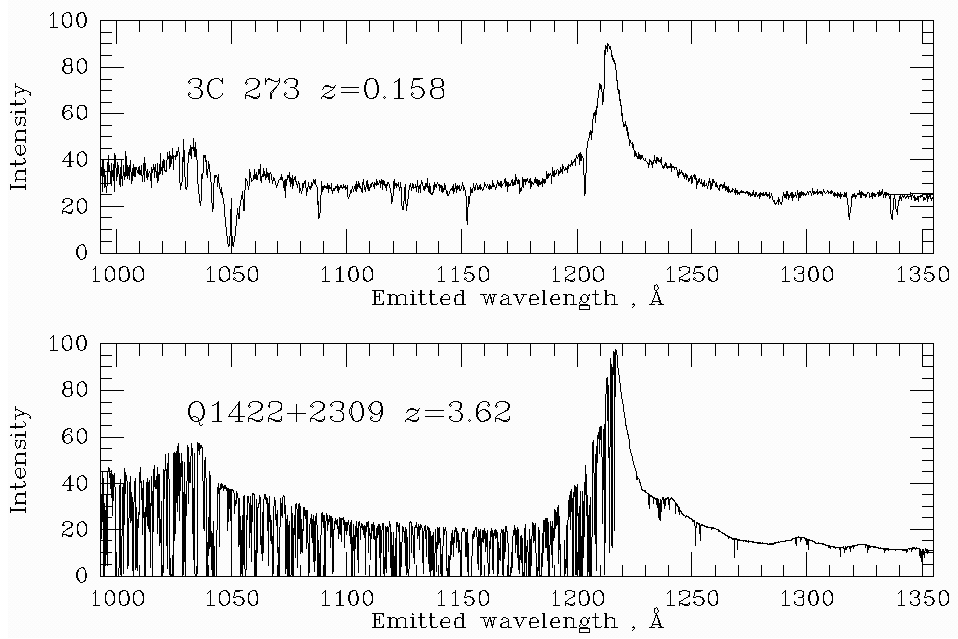
\includegraphics[width=0.7\textwidth]{../Images/forest.png}
			\caption{The spectra of two similar galaxies. Above: the spectrum of a galaxy at z=0.158 showing no significant extinction from Gunn Peterson scattering. Below: the spectrum of a galaxy at z=3.62 showing a Lyman forest caused by fluctuations in Hydrogen netrual fraction.}
			\label{fig:forest}
		\end{figure}

		It paradoxically seems, therefore, that the loss of flux caused by the Gunn-Peterson effect is extremely fortuitous to the observational cosmologist. Since the true emitted spectra of Lyman break galaxies are similar in nature to the spectra of closer galaxies with negligible Gunn Peterson absorption, it is possible, in theory, to probe the density of neutral Hydrogen at every point between the observed galaxy and the end of reionization.
	% subsection the_lyman_alpha_forest (end)

	\subsection{Properties of the Lyman Alpha line} % (fold)
	\label{sub:properties_of_the_lyman_alpha_line}
		The full relativistic equation for the energy levels of neutral Hydrogen was calculated by Dirac to be\cite{EisbergResnick}:
		\begin{align}
			E_{n,j} = - \frac{e^4}{ (4 \pi \epsilon_0)^2 2 \hbar^2 n^2} \left( \frac{m_p m_e}{m_p + m_e} \right) % E + R, p286
				\left [ 1 + \frac{\alpha^2}{n} \left( \frac{1}{j+1/2} - \frac{3}{4n} \right) \right]
		\end{align}
		Where n is the pricipal quantum number, j is the total spin eigenvalue and $\alpha$ is the fine structure constant:
		\begin{align}
			\alpha = \frac{e^2}{4 \pi \epsilon_0 \hbar c}  \approx \frac{1}{137}.
		\end{align}
		However, the final factor in square brackets is a small fractional correction of the order $10^{-5}$ or below and replacing the electron-proton reduced mass simply with the electron mass makes a fractional difference of the order of only $10^{-4}$. If both of these approximations are applied, the equation reduces to the more familiar relation for Hydrogen energy levels which can be derived from the Bohr model of quantum mechanics
		\begin{align}
			E_n = - \frac{m_e e^4}{8 \epsilon_0^2 h^2 n^2}.
		\end{align}
		Using this result, the energy transfer of the n=2 to n=1 transition can then be calculated
		\begin{align}
			\Delta E_{2,1} &= E_2 - E_1 = 10.199\si{\electronvolt} ,
		\end{align}
		corresponding to a wavelength of:
		\begin{align}
			\lambda_{Ly\alpha} = \frac{hc}{\Delta E_{2,1}} = 1215.7 \si{\angstrom}.
		\end{align}
		This means the absorbed photons will invariably be ultraviolet in the absorber rest frame, but for objects observed during the epoch of reionization, cosmological redshift will push the observed Lyman break into the near infrared in the observer frame. The challenges of observing these wavelengths from such large distances and potential methods of overcoming them comprise a large portion of this report.
	% subsection properties_of_the_lyman_alpha_line (end)

%%%% resonance graph

%%%% fan picture of the troughs

